\chapter{TBD}\label{chap:tbd}

Las imágenes satelitales son una fuente de información utilizadas cada vez mas en la actualidad por diferentes campos de la ciencia, a través de una imagen satelital podemos extraer información que permiten estudiar como por ejemplo las diferentes características del los suelos, obtener información de fenómenos naturales y ayudar a las toma de decisiones \ref{sec:estadodelarte}. Una cámara a bordo de un satélite además nos da la posibilidad de ayudar a la toma de decisiones en tiempo real logrando que de manera automática pueda por ejemplo trazar el curso del satélite previniendo coaliciones o como un mecanismo de ayuda para calibrar su apuntamiento (Sec:\ref{sec:fundamentacion}) brindando mas autonomía en la navegación y en la toma de decisiones. 

Como ya se menciono anteriormente en el  capitulo \ref{chap:introduccion} el objetivo de este trabajo de investigación  (Sec:\ref{sec:obj_general}) es realizar una evaluación experimental de factibilidad al utilizar algoritmos de aprendizaje automático para  la detección de patrones de interés de la misión  (Sec:\ref{sec:contexto})  brindando una  fuente extra de información al satélite para la toma de decisiones de manera automática. 

Los algoritmos de aprendizaje automático (Sec:\ref{sec:machinelaerning}) tienen la capacidad de generalizar (aprender)  a partir de los datos, estos datos son los que llamamos conjunto de entrenamiento, para entrenar (Sec:\ref{sub:aprendizaje}) un modelo de aprendizaje automático necesitamos además del conjunto de datos mencionados previamente, definir una función de costo (Sec:\ref{sub:funcion_costo}) que nos aproxime a los valores de la salida que estamos esperando y un algoritmo de clasificación (Sec:\ref{sub:clasificadores}) que nos indique a que clase o categoría pertenece cada valor. 

En el desarrollo de este trabajo no solo se preciso aprender realizar el entrenamiento de los datos también necesitamos extraer la información de la imagen. Para poder extraer la información de las imágenes utilizamos \textit{redes convolucionales} (Sec:\ref{sec:compueter-vision}), estas redes son una tipo de red que nos permiten extraer patrones (características) (Sec:\ref{sub:features-extraction}) de una imagen como el color, la forma, los bordes por medio de la operación de convolución (Sec:\ref{sub:convolucion}); las operaciones de convolución son operaciones de producto y sumas entre las diferentes capas y filtros de la red que generan como salida un mapa de característica que representa a la imagen. Existen en la actualidad diferentes arquitecturas de redes convolucionales como se desarrollo anteriormente en la sección (Sec:\ref{sub:arquitecturacnn}); mas adelante  detallaremos el tipo de arquitectura de red convolucional utilizada para este trabajo.

Uno de los problemas que se presentan a la hora de desarrollar un detector de patrones además de la extracción de la información de la imagen es determinar en que posición se encuentra el objeto de interés que deseamos reconocer esto se lo conoce en la literatura como el \textit{problema de la detección} (Sec:\ref{sub:problema_deteccion}), existen diferentes técnicas que nos ayudan a resolver este problema, estas técnicas son conocidas como \textit{regiones propuestas} (Sec:\ref{sub:regions-proposal}), algunas de estas son \textit{edges boxes} (Sec:\ref{sub:edgesboxes}), \textit{selective search} (Sec:\ref{sub:selectivesearch}), entre otras. Los métodos de regiones propuestas extraen y agrupan información de la imagen con similares característica, estos tipos de métodos generan un conjunto de regiones candidatas con una probabilidad en cada región generada que nos indica con que posibilidad pueda ser encontrado el objeto que estamos buscando en la imagen; cada región luego sera utilizada como conjunto de entrenamiento con algunos de los algoritmos de aprendizaje automático nombrado anteriormente. La salida de este\textit{esquema de procesamiento} será un modelo que permita detectar a que clase pertenece un nuevo dato nunca visto.

En este capítulo vamos a desarrollar el esquema de trabajo utilizado para la creación de un modelo de aprendizaje automático que permita detectar las zonas de interés como se expuso en la sección (Sec:\ref{sub:obj_especifico}). Además se describirá las diferentes metodologías y decisiones tomadas en la construcción de la solución como son las herramientas utilizadas, el etiquetado de los datos de entrenamiento, los diferentes  métodos de regiones propuestas utilizados, la arquitectura seleccionada para la extracción de las características de la imagen y por ultimo el proceso de clasificación y validación del modelo entrenado.




%En este capítulo vamos a detallar las decisiones tomadas en la selección de determinados métodos expuesto en el capítulo anterior, las  herramientas utilizadas y el tipo de arquitectura seleccionada para la extracción de los datos, es decir, se desarrollara el pipeline utilizado para la construcción de la solución.
%


\section{Esquema de Procesamiento}\label{sec: pipeline}

%En la siguiente imagen \ref{Fig:pipeline} podemos ver un pipeline de desarrollo en aprendizaje supervisado:
%\begin{figure}[H] \centering
%  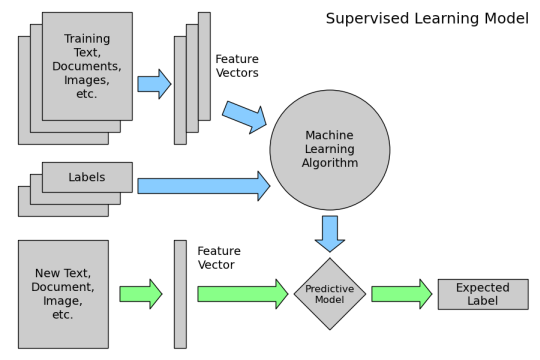
\includegraphics[height=8cm,keepaspectratio=true,clip=true]{imagenes/tbd/pipeline-sp.png}
%  \caption{Pipeline}\label{Fig:pipeline}
%\end{figure}
Partiendo de lo desarrollado anteriormente, en esta sección vamos a desarrollar el esquema de trabajo planteado para la solución del problema. En la siguiente figura \ref{Fig:pipeline-mio} se puede visualizar el \textit{pipeline} de trabajo realizado.

\begin{figure}[H] \centering
  \includegraphics[height=10cm,keepaspectratio=true,clip=true]{imagenes/tbd/pipeline_mio.png}
  \caption{Pipeline de Trabajo}\label{Fig:pipeline-mio}
\end{figure}

%https://www.datanami.com/2018/09/05/how-to-build-a-better-machine-learning-pipeline/
\subsection{Descripción del Pipeline desarrollado}\label{sub:desc-pipeline}

\subsubsection*{Datos Raw}
En esta etapa de trabajo se basó en recolectar todos los datos que serán usado para entrenar y validar el modelo, este proceso conlleva desde la descarga de los datos por medio de la pagina oficial de \ac{conae} hasta el almacenado de los mismos. En el sección \ref{sec:recoleccion} se desarrolla con mas detalle los pasos que se realizaron para la obtención y descarga de los datos.


%En esta parte del pipeline de desarrollo se trabajo desde la adquisición de los datos hasta llegar a la construcción del datasets de entrenamiento y test. La obtención de los datos se realizo a través de la pagina de \ac{conae} como se menciona en el capítulo \ref{chap:recoleccion}, para mas detalle ver  \ref{chap:anexo}. Las imágenes utilizadas son del sensor \ac{viirs}, estas imágenes están codificadas en un formato "h5",  \textit{Hierarchical Data Format}, este formato es el utilizado para almacenar datos de gran tamaño; cada banda del sensor se la almacena para ser luego procesada y crear la imagen.

%
\subsubsection*{Preprocesamiento}

A partir de los datos descargados en el paso anterior se debe realizar el procesamiento de los mismos para poder utilizarlo; este procesamiento se basa en convertir los datos \textit{raw} en imágenes. El proceso de conversión de datos en imágenes se realizo a través de la herramienta \textit{ENVI} \ref{sub:enviSoft}, esta herramienta es un software  especializado en el procesamiento y análisis de imágenes  geoespaciales.

Debido a la característica que posee el sensor que utilizamos en el desarrollo ,\textit{VIIRS}, se descompone en diferentes bandas en el espectro electromagnético de las cuales seis bandas son relacionadas en el espectro visible (\textit{VIS}), cuatro en el infrarrojo cercano (\textit{NIR} por sus siglas en inglés), cuatro en el infrarrojo de onda corta (\textit{SWIR}), tres en el infrarrojo medio (\textit{MIR}) y cuatro en el infrarrojo térmico (\textit{TIR}). Para la construcción del set de datos final se usaron diferentes combinaciones de bandas (Sec:\ref{sub:comb_de_banda}), cada una de las bandas deben ser cargadas al software \textit{ENVI} que luego se combinaran cada una de estas en diversos canales \textit{RGB} para la construcción de la misma. Luego de este proceso obtenemos la imagen final como se puede visualizar en la siguiente figura \ref{Fig:img-final}.

En el sección \ref{sec:recoleccion} se desarrolla de manera mas detallada que bandas bandas fueron utilizadas y el proceso que se llevo a cabo para conversión de datos.

\begin{figure}[H] \centering
  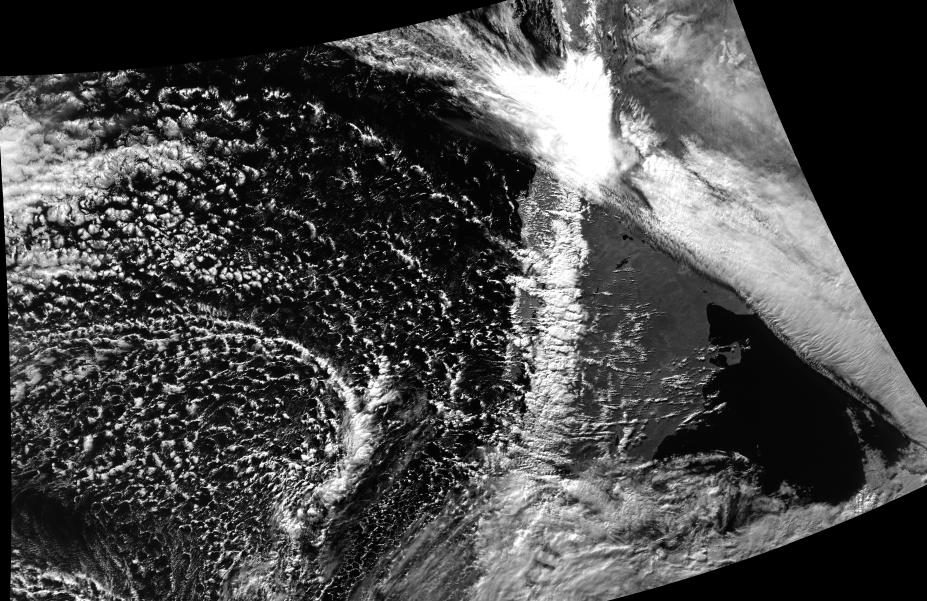
\includegraphics[height=9cm,keepaspectratio=true,clip=true]{imagenes/tbd/pre-img.png}
  \caption{Imagen final obtenida luego del procesamiento.}\label{Fig:img-final}
\end{figure}


\subsubsection*{Regions Proposal}

Una vez obtenida las imágenes se generó regiones candidatas a través de métodos de regiones propuestas (Sec:\ref{sub:regions-proposal}) como se pude visualizar en la siguiente imagen \ref{Fig:rp-ejemplo}, estos conjunto de métodos nos retorna  un conjunto de \textit{bounding boxes} dentro de la imagen.
%coordenadas ($x$, $y$) al que pertenece dentro de la imagen. 

\begin{figure}[H] \centering
  \includegraphics[height=9cm,keepaspectratio=true,clip=true]{imagenes/tbd/proposal-img.png}
  \caption{Ejemplo regions proposal}\label{Fig:rp-ejemplo}
\end{figure}



En base a los diferentes métodos desarrollados en la sección (Sec:\ref{sub:regions-proposal}) se realizo una evaluación empírica de los mismos. Para dar mas detalle de la evaluación realizada podemos ver la siguiente tabla \ref{tabla:comparacionregiones}:


%Se realizo una evaluación empírica de que método seleccionar para el desarrollo en la siguiente tabla se desarrolla el análisis realizado \ref{tabla:comparacionregiones}:

\begin{table}[H]\centering
\begin{tabular}{|p{2cm}|p{6cm}|p{8cm}|}
    \hline 
     \centering \textbf{Método}  & \centering \textbf{Ventajas} & \multicolumn{1}{c|}{\centering \textbf{Desventajas}} \\
    \hline
    \centering Selective Search \ref{sub:selectivesearch} & \parbox[p][0.2\textwidth][c]{6cm}{
    \begin{itemize}
        \item Extrae la probabilidad de que exista un objeto en la región encontrada.
        \item Diferentes escalas de detección.
        \item Se puede customizar el tamaño de cada región.
    \end{itemize}}  &  \parbox[p][0.2\textwidth][c]{7.5cm}{
    \begin{itemize}
        \item Tiempo de ejecución muy alto para imágenes de resolución mayores; ejemplo: 2800x3000px.	
    \end{itemize} } \\ \hline
    \centering Edges Boxes \ref{sub:edgesboxes} & \parbox[p][0.2\textwidth][c]{6cm}{
    \begin{itemize}
        \item Buen tiempo de ejecución con imágenes de gran tamaño
        \item Reconocimientos de regiones de menor tamaño
        \item Nos da la probabilidad de que la región contenga un objeto.
    \end{itemize} } & \parbox[p][0.2\textwidth][c]{7.5cm}{
    \begin{itemize}
        \item No segmenta las regiones, por lo que pierde precisión en relación a métodos como selective search.
    \end{itemize} } \\ \hline 
     \centering BING & \parbox[p][0.2\textwidth][c]{6cm}{
    \begin{itemize}
        \item Tiempo de ejecución.
    \end{itemize} } &  \parbox[p][0.2\textwidth][c]{7.5cm}{
    \begin{itemize}
        \item No encuentra regiones cuando las imágenes son grandes.
        \item No se puede customizar el tamaño de la ventana
    \end{itemize} } \\ \hline
\end{tabular}
\caption{Análisis de métodos Regiones Propuestas}
\label{tabla:comparacionregiones}
\end{table}

\subsubsection*{Non-maximums Suppression}

En esta etapa del \textit{pipeline} una vez obtenido el conjunto de regiones candidatas por cada una de las imágenes se aplicó \ac{nms} (Sec:\ref{sub:nonmaximumsuppression}) para descartar regiones con sobre muestreo quedándonos solo con aquellas regiones que cumplen determinado criterio de solapamiento definido, \textit{IoU}, intersección sobre unión, en este caso el umbral utilizado para eliminar regiones fue de 80\%. Este proceso se realizo para cada una de las imágenes del set de datos descargado.


\subsubsection*{Extracción de características}
Luego del proceso de \ac{nms} para cada región obtenida se debe extraer la información de cada una de las imágenes. Las redes neuronales convolucionales (Sec:\ref{sub:cnn}), permiten extraer las característica distintiva de la imagen haciendo uso de operaciones de convolución como se desarrollo en el capítulo (Sec:\ref{sub:cnn}). El proceso de extracción de información consta como primer paso seleccionar el tipo de arquitectura de la red que sera utilizada, para esta tesis se trabajo con \textit{ResNet50} (Sec:\ref{sub:arquitecturacnn}), la arquitectura  resnet50 recibe como input una imagen de $224 x 224$ y nos retorna un vector de 2048 que sera nuestro input para el entrenamiento del modelo.
Como paso siguiente luego de la selección de la arquitectura se debe normalizar las imágenes al tamaño requerido por la red; esta imagen normalizada será convertida a un vector que pasara por cada una de las capas de la red ,\textit{convolucion}, \textit{polling}, \textit{fully conected}; para luego ser extraída de la ante ultima capa que sera la que contenga la información final de la imagen.

El proceso descripto anterior se debe realizar para cada una de los bounding boxes contenidos en la imagen.



%extrajo la información de cada región utilizando redes neuronales convolucionales \ref{sub:cnn}, para esto utilizamos redes pre-entrenadas \ref{sub:arquitecturacnn}. 

%El proceso de extracción se basa en dada una imagen de entrada luego que pasa por toda la red extraer la capa anterior a la ultima, esto lo hacemos porque esta capa tiene toda la información de las característica de la imagen que logro aprender. La información extraída tiene la forma de un vector de $N$ dimensiones dependiendo la arquitectura de la red pre-entrenada que estemos usando, en esta tesis la arquitectura utilizada para el proceso de extracción de característica es una \textit{ResNet50}, obteniendo un vector 2048 elementos como salida de la red.

%Una vez obtenido los vectores de cada región de toda la imagen se %almacenaron en un archivo \textit{.mat} para luego entrenar un %clasificador con ellos.


\subsubsection*{Generación de datos para entrenamiento}

Dado en que estamos por entrenando un algoritmo de aprendizaje supervisado debemos tener las etiqueta de cada región. Para poder crear el datasets debemos tener identificado nuestras regiones de interés es decir el \textit{ground thruth} que vamos a utilizar. Las regiones de interés, como se menciona en la sección (Sec:\ref{sec:obj_general}), son el \textit{Golfo de San Matias} y la \textit{Laguna de Mar Chiquita}; la locación de cada región de interés se marco utilizando la librería \textit{Labelme} (Sec:\ref{sec:instalacionlabelme}), este es un proceso manual que se debe realizar con cada unas de las imágenes marcando con polígonos las regiones, como se puede ver en la siguiente imagen \ref{Fig:labelme-etiquetado}. El polígono de la región de interés es almacenado en un formato \textit{json}, que luego sera utilizado para compararse con las regiones candidatas obtenidas por algunos de los métodos de regiones propuestas. 


En el proceso de etiquetado debemos usar las anotaciones (polígonos) de nuestro \textit{ground thruth} y los regions proposal obtenidos por algunos de los métodos mencionados anteriormente; con estas dos regiones se calcula \textit{IoU}, intersección sobre unión, si el valor del \textit{IoU} superaba el 80\% entonces esa región se la identifica como clase positiva, en caso contrario se marca la región como clase negativa, este proceso se realizo por cada una de las regiones obtenidas de cada una de las imágenes.

%Para realizar el etiquetado de los datos se debe calcular \textit{IoU}, intersección sobre unión, entre la región candidata y las regiones de interés etiquetada previamente con la librería \textit{Labelme}, 

\begin{figure}[H] \centering
  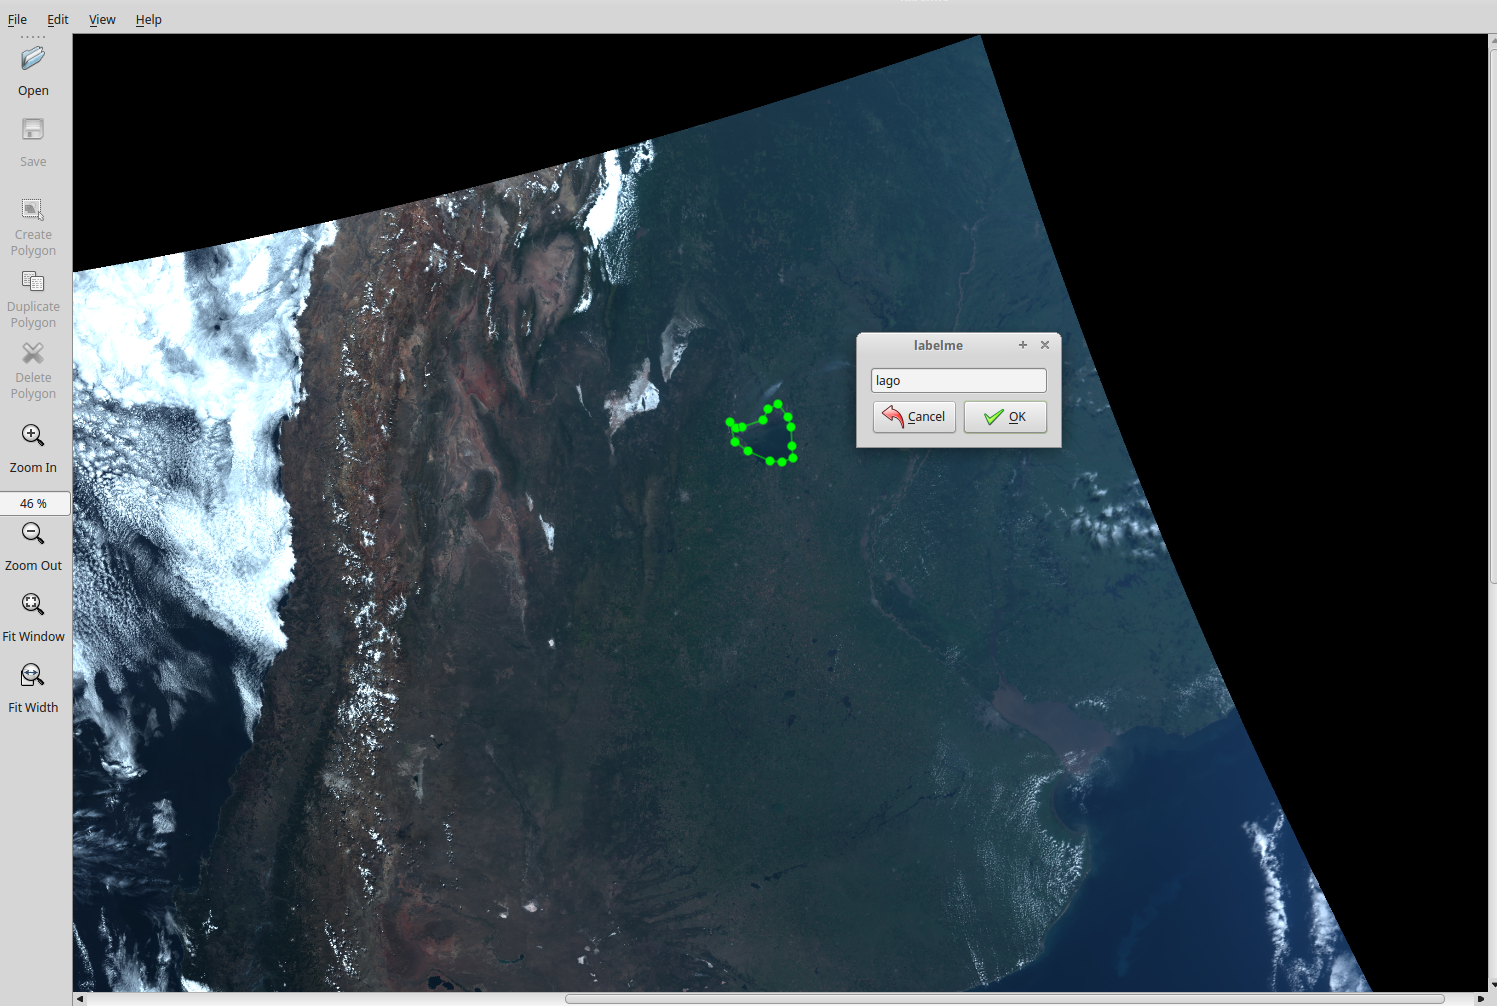
\includegraphics[height=9cm,keepaspectratio=true,clip=true]{imagenes/tbd/labelme1.png}
  \caption{Ground Thruth - etiquetado}\label{Fig:labelme-etiquetado}
\end{figure}

Cada uno de los datos etiquetados están relacionado a uno de los vectores de característica extraído anteriormente, luego de realizar todo el proceso de extracción y etiquetado ya tenemos el datasets final con el que vamos a entrenar el modelo.


%Con el el dataset de train se realizo el entrenamiento del modelo %utilizando \textit{grid search} como algoritmo de búsqueda de %hiper-parámetros del modelo \textit{SVM} \ref{sub:clasificadores} y %\textit{cross validation} \ref{Fig: crossvalidation} para evitar %problemas de \textit{overfitting} \ref{sub:problema_deteccion}.


\subsubsection*{Evaluación}

La validación de los datos como se nombro anteriormente se realizo con el datasets de test de la cual se calculo las métricas de \textit{precision}, \textit{recall} y \textit{auroc} (Sec:\ref{sub:evaluación-modelo}) para medir la eficiencia de los  modelos entrenados en el paso anterior. Luego de diversas iteraciones se llegó a un modelo que maximicen estas métricas mencionadas, este modelo sera la versión final que será utilizado para realizar la predicción de datos que nunca vio el modelo.

La predicción del modelo final tendrá como respuesta un conjunto de regiones (x, y) de la imagen nueva de entrada en el cual cada una de estas regiones esta asociada una respuesta que nos indica con los valor "0" si la región de interés no se encuentra en la imagen en caso contrario  retornara "1"; cada una de esta predicciones esta asociada a un valor de probabilidad que indica cuan posible es que la región de interés buscada este en esa imagen.

\section{Recolección de Datos}\label{sec:recoleccion}

En este capítulo se describirá  los pasos que se llevaron a cabo para obtener los datos de la tesis. Se  desarrollara de manera mas detallada como se obtuvo el dataset y que configuraciones de bandas se usaron para la construcción de las imágenes.


\subsection{Imágenes Satelitales}

Una imagen satelital se la puede definir como la representación visual de información capturada por un sensor montado en un satélite artificial (Sec:\ref{sub:imagen_satelital}). Estos sensores recogen la información reflejada por la superficie de la tierra que luego es enviada para su posterior procesamiento.

El uso de imágenes satelitales constituye una excelente herramienta para el conocimiento y monitoreo de los territorios y recursos; hoy en día disfrutamos de la oportunidad de aprovechar estas imágenes satelitales para una gran variedad de aplicaciones como: desarrollo y planificación urbana, infraestructura, recursos naturales, investigación, alerta temprana de catástrofes, asuntos militares, entre otras.

Una imagen satelital debe pasar por diferentes niveles de procesamiento dependiendo el tipo de uso que se le quiera dar, en la siguiente sección (Sec:\ref{sub:nivelesdeprocesamiento}) se desarrolla mas en detalle.

\subsubsection{Niveles de procesamiento}\label{sub:nivelesdeprocesamiento}

En el campo de la teledeteccion (Sec:\ref{sub:teledeteccion}) cuando hablamos de niveles de procesamiento nos referimos a los diversos procesos que son aplicados a una imagen satelital. Dependiendo de la agencia espacial existe una nomenclatura para determinar que niveles de procesamiento fueron aplicados.

En este trabajo se utilizo la nomenclatura propuesta por \ac{nasa}:
\begin{itemize}
	\item \textbf{Nivel 0}: La información científica recogida está a máxima resolución, ordenada temporalmente y con errores de transmisión, artefactos y duplicados eliminados.
 	\item \textbf{Nivel 1a}: La información esta ordenada cronológicamente y datos auxiliares como coeficientes de calibración y parámetros de referencia.
 	\item \textbf{Nivel 1b}: La información del 1a es procesada a unidades de detección, geo-refereciada.
 	\item \textbf{Nivel 2}: Variables geofísicas derivadas por ejemplo productos de concentraciones de hielo, ola de mar, etc.
 	\item \textbf{Nivel 3}: Las variables son mapeadas uniformemente en \textit{grids} espacio-temporales.
 	\item \textbf{Nivel 4}: Resultados de los análisis de los niveles anteriores
\end{itemize}


\subsection{Datos raw}\label{sec:datosutilizados}

Los datos utilizados para el desarrollo de los experimentos fueron descargadas por medio del catalogo  publicado en el sitio oficial de \ac{conae} \footnote{Fuente: http://catalogos.conae.gov.ar/catalogo/catalogo-de-imagenes.html} de acceso gratuito para el publico. Se debe señalar además que se trabajó con imágenes correspondiente a los años 2017 y 2018 con una ventana de tiempo desde Abril del 2017 a Marzo del 2018; estas imágenes son de naturaleza óptica con un nivel de procesamiento \textbf{1a}, de acuerdo a las nomenclaturas utilizadas en la sección (Sec:\ref{sub:nivelesdeprocesamiento}).

De acuerdo a las característica del proyecto y tomando como fundamentación lo expuesto en la sección (Sec:\ref{sec:fundamentacion}), se utilizaron imágenes que se asemejan a las características del \ac{fs} \ac{conae} detalladas en los requerimientos formales del mismo; estas imágenes fueron adquiridas por el instrumento \ac{viirs} (Sec:\ref{sub:viirs}) a bordo del satélite Suomi-NPP.


Para la realización de diversos experimentos se utilizaron en total 29 combinaciones de bandas \ref{tab:combinacion_banda}, contando con 50 imágenes por cada combinación de bandas que se realizo.


\subsubsection{Instrumento VIIRS}\label{sub:viirs}
El instrumento \ac{viirs} fue lanzado a bordo del satélite Suomi-NPP el 28 de octubre de 2011. Este instrumento posee 5 canales de alta resolución (I-bands), 16 canales de resolución moderada (M-bands) y un canal de baja luz (Day/Night Band, DNB).  En el siguiente cuadro se detallan las diferentes longitudes de onda y los rangos de onda de las bandas, junto con resolución geométrica apuntando a Nadir (ver tabla: \ref{tab:viirs}).
\begin{table}[H]
\begin{center}
\begin{tabular}{|c|c|c|}
\hline Banda & Rango Espectral (um) & Resolución Nadir \\\hline 
 		M1  & 0.402-0.422   & 0.742 x 0.259 \\ \hline 
		M2  & 0.436-0.454   & 0.742 x 0.259 \\ \hline 
		M3  & 0.478-0.498   & 0.742 x 0.259 \\ \hline 
		M4  & 0.545-0.565   & 0.742 x 0.259 \\ \hline 
		I1  & 0.600-0.680   & 0.371 x 0.387 \\ \hline 
		M5  & 0.662-0.682   & 0.742 x 0.259 \\ \hline 
		M6  & 0.739-0.754   & 0.742 x 0.776 \\ \hline 
		I2  & 0.846-0.885   & 0.371 x 0.387 \\ \hline 
		M7  & 0.846-0.885   & 0.742 x 0.259 \\ \hline 
		M8  & 1.230-1.250   & 0.742 x 0.776 \\ \hline 
		M9  & 1.371-1.386   & 0.742 x 0.776 \\ \hline 
		I3  & 1.580-1.640   & 0.371 x 0.387 \\ \hline 
		M10 & 1.580-1.640   & 0.742 x 0.776 \\ \hline 
		M11 & 2.225-2.275   & 0.742 x 0.776 \\ \hline 
		I4  & 3.550-3.930   & 0.371 x 0.387 \\ \hline 
		M12 & 3.660-3.840   & 0.742 x 0.776 \\ \hline 
		M13 & 3.973-4.128   & 0.742 x 0.259 \\ \hline 
		M14 & 8.400-8.700   & 0.742 x 0.776 \\ \hline 
		M15 & 10.263-11.263 & 0.742 x 0.776 \\ \hline 
		I5  & 10.500-12.400 & 0.371 x 0.387 \\ \hline 
		M16 & 11.538-12.488 & 0.742 x 0.776 \\ \hline 
\end{tabular}
\end{center}\caption{Característica de bandas,\ac{viirs} \label{tab:viirs}}
\end{table}

\subsubsection{Combinaciones de bandas en canales RGB}\label{sub:comb_de_banda} 
%http://www.gisandbeers.com/combinacion-de-imagenes-satelite-landsat-sentinel-rgb/

Las redes neuronales que vamos a utilizar para la construcción de esta tesis son redes neuronales pre-entrenadas (Sec:\ref{sub:cnn}), estas redes neuronales necesitan como entrada imágenes ópticas con tres canales correspondiente a \textit{RGB} (rojo, verde y azul), los canales RGB se emplean para representar distintos colores a partir de la mezcla de cada uno de estos.

Para construir el dataset de entada a la red se debió convertir los datos \textit{raw} en imágenes tomando como base los canales RGB mencionados. Las combinaciones de bandas en imágenes satelitales nos ayudan a analizar diferentes elementos dentro de la misma imagen, para esto utilizamos diversas combinaciones de bandas en cada canal RGB que que nos muestran diferentes elementos de acuerdo a la banda utilizada. El paso de cada banda por un canal RGB especifico permitirá teñir de colores los elementos que ofrezcan mayor o menor reflexión de longitudes de onda como por ejemplo, la vegetación, focos de incendios, entre otros brindando diversa fuente de información para ser explorada. 

En el siguiente cuadro  \ref{tab:combinacion_banda} se puede ver todas las combinaciones de bandas utilizadas para la construcción del dataset. El conjunto de bandas seleccionadas para los experimentos son las de resolución moderada (M-bands) \ref{tab:viirs} , que posee una resolución espacial a nadir de 750 metros.

\begin{table}[H] \begin{center}
\begin{tabular}{|c|c|}\hline 
Num & Combinación de banda\\ \hline 
1  	& 	M1-M1-M1 	\\ \hline
2  	&   M1-M3-M5	\\  \hline
3  	& 	M1-M5-M3	\\ \hline
4  	&   M3-M1-M5 	\\ \hline
5   & 	M3-M3-M3 	\\ \hline
6   & 	M3-M5-M1 	\\ \hline
7   & 	M5-M1-M3 	\\ \hline
8   & 	M5-M3-M1 	\\ \hline
9   &   M5-M5-M5  	\\ \hline
10  &	M7-M7-M7   	\\ \hline
11  & 	M9-M9-M9   	\\ \hline
12  & 	M11-M7-M9  	\\ \hline
13  & 	M11-M9-M7  	\\ \hline
14  &  	M7-M11-M9  	\\ \hline
15  & 	M7-M9-M11  	\\ \hline
16  & 	M9-M11-M7  	\\ \hline
17  & 	M9-M7-M11  	\\ \hline
18  & 	M11-M11-M11	\\ \hline
19  & 	M11-M13-M15 \\ \hline
20  & 	M11-M15-M13 \\ \hline
21  & 	M13-M11-M15 \\ \hline
22  & 	M13-M13-M13	\\ \hline
23  & 	M13-M15-M11 \\ \hline
24  & 	M15-M11-M13	\\ \hline
25  & 	M15-M13-M11	\\ \hline
26  & 	M15-M15-M15 \\ \hline
27  & 	M5-M4-M3 	\\ \hline
28  & 	M10-M7-M5 	\\ \hline   
29  & 	M11-M12.M13	\\ \hline        	
\end{tabular}
\end{center}\caption{Combinaciones de bandas utilizadas \label{tab:combinacion_banda}}
\end{table}

En la siguiente figura \ref{Fig: bandas543} podemos visualizar unas de las imágenes que se utilizo; en este caso corresponde  a las combinaciones de bandas M5, M4, M3 conocidas como color verdadero, \textit{true color} su nombre en ingles .

\begin{figure}[H]
 \centering
  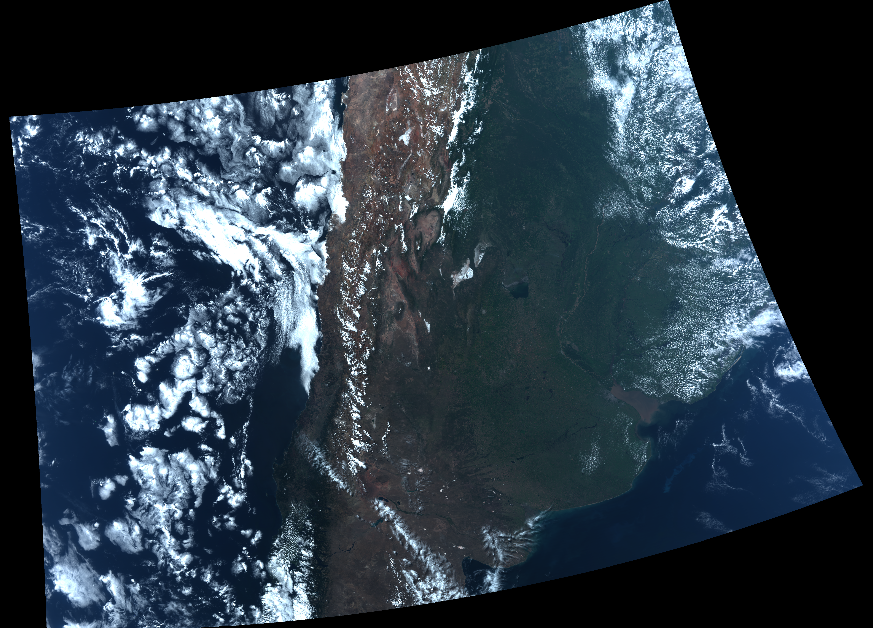
\includegraphics[height=10cm,keepaspectratio=true,clip=true]{imagenes/recoleccion/img-543.png}
  \caption{Combinación de bandas M5, M4 y M3}
	\label{Fig: bandas543}
\end{figure}

